% Options for packages loaded elsewhere
\PassOptionsToPackage{unicode}{hyperref}
\PassOptionsToPackage{hyphens}{url}
\PassOptionsToPackage{dvipsnames,svgnames,x11names}{xcolor}
%
\documentclass[11pt]{article}
\usepackage{amsmath,amssymb}
\usepackage{lmodern}
\usepackage{iftex}
\ifPDFTeX
  \usepackage[T1]{fontenc}
  \usepackage[utf8]{inputenc}
  \usepackage{textcomp}
\fi
\IfFileExists{microtype.sty}{\usepackage[]{microtype}\UseMicrotypeSet[protrusion]{basicmath}}{}
\makeatletter
\@ifundefined{KOMAClassName}{%
  \IfFileExists{parskip.sty}{\usepackage{parskip}}{%
    \setlength{\parindent}{0pt}\setlength{\parskip}{6pt plus 2pt minus 1pt}}
}{\KOMAoptions{parskip=half}}
\makeatother
\usepackage{xcolor}
\IfFileExists{xurl.sty}{\usepackage{xurl}}{}
\IfFileExists{bookmark.sty}{\usepackage{bookmark}}{\usepackage{hyperref}}
\hypersetup{
  pdftitle={Energy-aware ventilation for the LTU A-house, Architecture Document},
  pdfauthor={Kasper Axelsson, Mohamd Amar Chms Aldden},
  colorlinks=true,
  linkcolor={RoyalBlue},
  filecolor={Maroon},
  citecolor={Blue},
  urlcolor={Blue}}
\urlstyle{same}
\usepackage[a4paper,margin=2.4cm]{geometry}
\usepackage{longtable,booktabs,array}
\usepackage{calc}
\usepackage{graphicx}
\makeatletter
\def\maxwidth{\ifdim\Gin@nat@width>\linewidth\linewidth\else\Gin@nat@width\fi}
\def\maxheight{\ifdim\Gin@nat@height>\textheight\textheight\else\Gin@nat@height\fi}
\makeatother
\setkeys{Gin}{width=\maxwidth,height=\maxheight,keepaspectratio}
\setlength{\emergencystretch}{3em}
\providecommand{\tightlist}{\setlength{\itemsep}{0pt}\setlength{\parskip}{0pt}}
\setcounter{secnumdepth}{-\maxdimen}
\usepackage{newunicodechar}
\usepackage{textcomp}
\usepackage{amssymb}
\newunicodechar{°}{\textdegree}
\newunicodechar{₂}{\textsubscript{2}}
\newunicodechar{→}{\ensuremath{\rightarrow}}
\newunicodechar{≤}{\ensuremath{\leq}}
\newunicodechar{≥}{\ensuremath{\geq}}
\newunicodechar{≈}{\ensuremath{\approx}}
\newunicodechar{✓}{\ensuremath{\checkmark}}
\newunicodechar{–}{--}
\newunicodechar{—}{---}
\usepackage{etoolbox}
\AtBeginEnvironment{longtable}{\footnotesize}
\AtBeginEnvironment{tabular}{\footnotesize}
\usepackage{fancyhdr}
\pagestyle{fancy}\fancyhf{}
\rhead{\small D7065E\,--\,Architecture Document}
\lhead{\small Energy-aware ventilation, final report}
\cfoot{\thepage}
\renewcommand{\headrulewidth}{0.4pt}
\usepackage{titlesec}
\titleformat{\section}{\Large\bfseries}{\thesection}{0.6em}{}
\titleformat{\subsection}{\large\bfseries}{\thesubsection}{0.5em}{}
\usepackage{microtype}
\usepackage{pgfplots}
\pgfplotsset{compat=1.16}
\setlength{\emergencystretch}{2em}

\newcommand{\cotwo}{CO\textsubscript{2}}
\usepackage{caption}
\captionsetup{font=small,labelfont=bf,skip=4pt}
\setlength{\LTpre}{4pt}\setlength{\LTpost}{6pt}

% A figure centred on the page at a width that may exceed the text block. The
% large diagrams need it for their labels to print at a readable size.
\newcommand{\widefigure}[2][1.12]{\par\noindent\makebox[\linewidth][c]{\includegraphics[width=#1\linewidth]{#2}}\par}
% The same with a line of text under it that stays on the figure's page.
\newcommand{\widefigurewithnote}[3][1.12]{\par\noindent\begin{minipage}{\linewidth}\centering
  \makebox[\linewidth][c]{\includegraphics[width=#1\linewidth]{#2}}\\[4pt]{\small #3}\end{minipage}\par}

\begin{document}

\begin{center}
{\LARGE Energy-aware ventilation for the LTU A-house\par}
\vspace{0.4em}
{\large D7065E, Architecture Document\par}
\vspace{0.6em}
{Kasper Axelsson \& Mohamd Amar Chms Aldden\par}
\end{center}

{\hypersetup{linkcolor=black}\setcounter{tocdepth}{1}\small\tableofcontents}

\section{1. Summary}

The system ventilates and heats 50 rooms of the A-house in BuildSim according to who is in
them. A controller reads \cotwo, temperature and a people count from sensor devices,
forecasts each room's occupancy from a learned time-of-day profile, and commands a damper
and a radiator valve per room. One principle runs through the design: \textbf{the
controller proposes, the building disposes.} The controller knows the building only
through what sensor devices report, and every safety limit is enforced in the actuator,
which keeps working when the controller, the broker or a sensor does not. Over a
simulated week the system holds \cotwo{} under 1000\,ppm in every occupied minute for
57\,\% less energy than ventilation on a time clock.

\begin{longtable}[]{@{}>{\raggedright\arraybackslash}p{0.22\linewidth}>{\raggedright\arraybackslash}p{0.72\linewidth}@{}}
\toprule
\textbf{Project title} & Energy-aware ventilation and climate control for the LTU A-house \\
\textbf{Team members} & Kasper Axelsson, Mohamd Amar Chms Aldden \\
\textbf{Use case} & Demand-controlled ventilation with occupancy prediction \\
\textbf{Repository} & \url{https://github.com/MisterD0ctor/d7065e-project} (design notes, contracts, test plan and review log in \texttt{docs/}) \\
\textbf{Version / date} & 2026-10-11 \\
\bottomrule
\end{longtable}

\textbf{Changes since the proposal.}
(1) \emph{Occupancy is measured, not estimated.} The proposal inverted the \cotwo{} mass
balance to estimate head-count; for lack of time each room has a people counter instead,
the fallback the proposal named. The mass balance survives as a plausibility check on that
counter (Section 7.1). (2) \emph{The data path was rebuilt on 10 October.} We had read
``the controller must not see the truth'' as ``the truth must not enter BuildSim'' and
built a truth API beside BuildSim. That is not the lab's architecture; the system now
follows the quickstart, with BuildSim in the middle (Section 4.4, D-12). All results in
this report were measured after that change. (3) \emph{The baseline is a time clock}, not
design flow around the clock, which no building runs at night and which had inflated the
saving from 57\,\% to 75\,\%.

\section{2. Use case and building context}

BuildSim holds the A-house: the floor plan, equipment with sensor values and actuator
states, the people, and a 3D viewer. It stores current state only; it simulates no
physics, keeps no history and has no clock. The course's occupancy simulator fills it with
staff, students and night guards following a seeded daily plan. We chose 50 rooms on
level 0: 3 common (fika) rooms, 20 lecture rooms and 27 small rooms, 24 of them in use as offices.

Ventilating by a schedule wastes energy on empty rooms and still under-ventilates full
ones. Ventilating by measured \cotwo{} reacts only after the air has degraded, and a
room's air responds slowly (time constant 12 to 60 minutes). The objective is to keep
\cotwo{} below 1000\,ppm and temperature within 20--24\,\textdegree C while anyone is in a
room, for as little fan and heating energy as possible, and to stay safe when a sensor,
the controller or the network fails.

\section{3. Requirements}

\begin{longtable}[]{@{}>{\raggedright\arraybackslash}p{0.07\linewidth}>{\raggedright\arraybackslash}p{0.66\linewidth}>{\raggedright\arraybackslash}p{0.19\linewidth}@{}}
\toprule
\textbf{ID} & \textbf{Requirement} & \textbf{Verified by} \\
\midrule
\endhead
FR-1 & A physical model simulates \cotwo{} and temperature per room, first order, driven by true occupancy and the airflow and setpoint the actuators have reached; steps $\leq$ 1 model minute & T-01, T-41 \\
FR-2 & Each room has a \cotwo, a temperature and an occupancy sensor device; each reports once per model minute with noise: \cotwo{} $\pm$(30\,ppm + 3\,\%), temperature $\pm$0.3\,\textdegree C, count $\pm$1 & T-03, T-41, T-42 \\
FR-3 & The controller sets airflow and heating setpoint for every room once per minute & T-05 \\
FR-4 & It forecasts each room's occupancy one lead time ahead from a model trained offline & T-06, T-35 \\
FR-5 & The actuator validates every command (range, unit, TTL, duplicate) and travels at a fixed rate & T-07, T-08 \\
FR-6 & Safety in the damper, independent of the controller: \cotwo{} $>$ 1100\,ppm gives maximum flow; never below 0.35\,l/s\,m\textsuperscript{2} in occupied hours, 0.10 otherwise & T-09, T-10, T-11 \\
FR-7 & A stale or stuck sensor is detected and the room falls back: design flow without \cotwo, 21\,\textdegree C without temperature, forecast and \cotwo{} without the count & T-12, T-13, T-36--38 \\
FR-8 & Every reading, true value, command and decision is stored with model time and run id & T-14, T-43 \\
FR-9 & Four policies selectable by a flag; nothing else differs between runs & T-15, T-32 \\
FR-10 & A dashboard shows each room and the building, now and over time, with alerts & T-16, T-39 \\
FR-11 & Devices do nothing until an installer has registered them; BuildSim's equipment is restored after a restart & T-17, T-28--31 \\
\midrule
NFR-1 & \cotwo{} $\leq$ 1000\,ppm for $\geq$ 95\,\% of occupied room-minutes & T-18 \\
NFR-2 & 20--24\,\textdegree C for $\geq$ 95\,\% of occupied room-minutes & T-19 \\
NFR-3 & Energy $\geq$ 30\,\% below the scheduled baseline & T-20 \\
NFR-4 & A command shows in the damper's state within one model minute (95th percentile) & T-21 \\
NFR-5 & 50 rooms: every sensor's reading arrives every model minute & T-22, T-42 \\
NFR-6 & Any one of our processes can be lost without an unsafe state; the loop resumes within 30\,s & T-23, T-24, T-40 \\
NFR-7 & Same seed and date give identical occupancy; every number traces to a run id & T-25 \\
NFR-8 & One baseline over five simulated weekdays in $\leq$ 2.5\,h & T-26 \\
\bottomrule
\end{longtable}

\section{4. Architecture}

\subsection{4.1 Context diagram (C4 Level 1)}

\begin{center}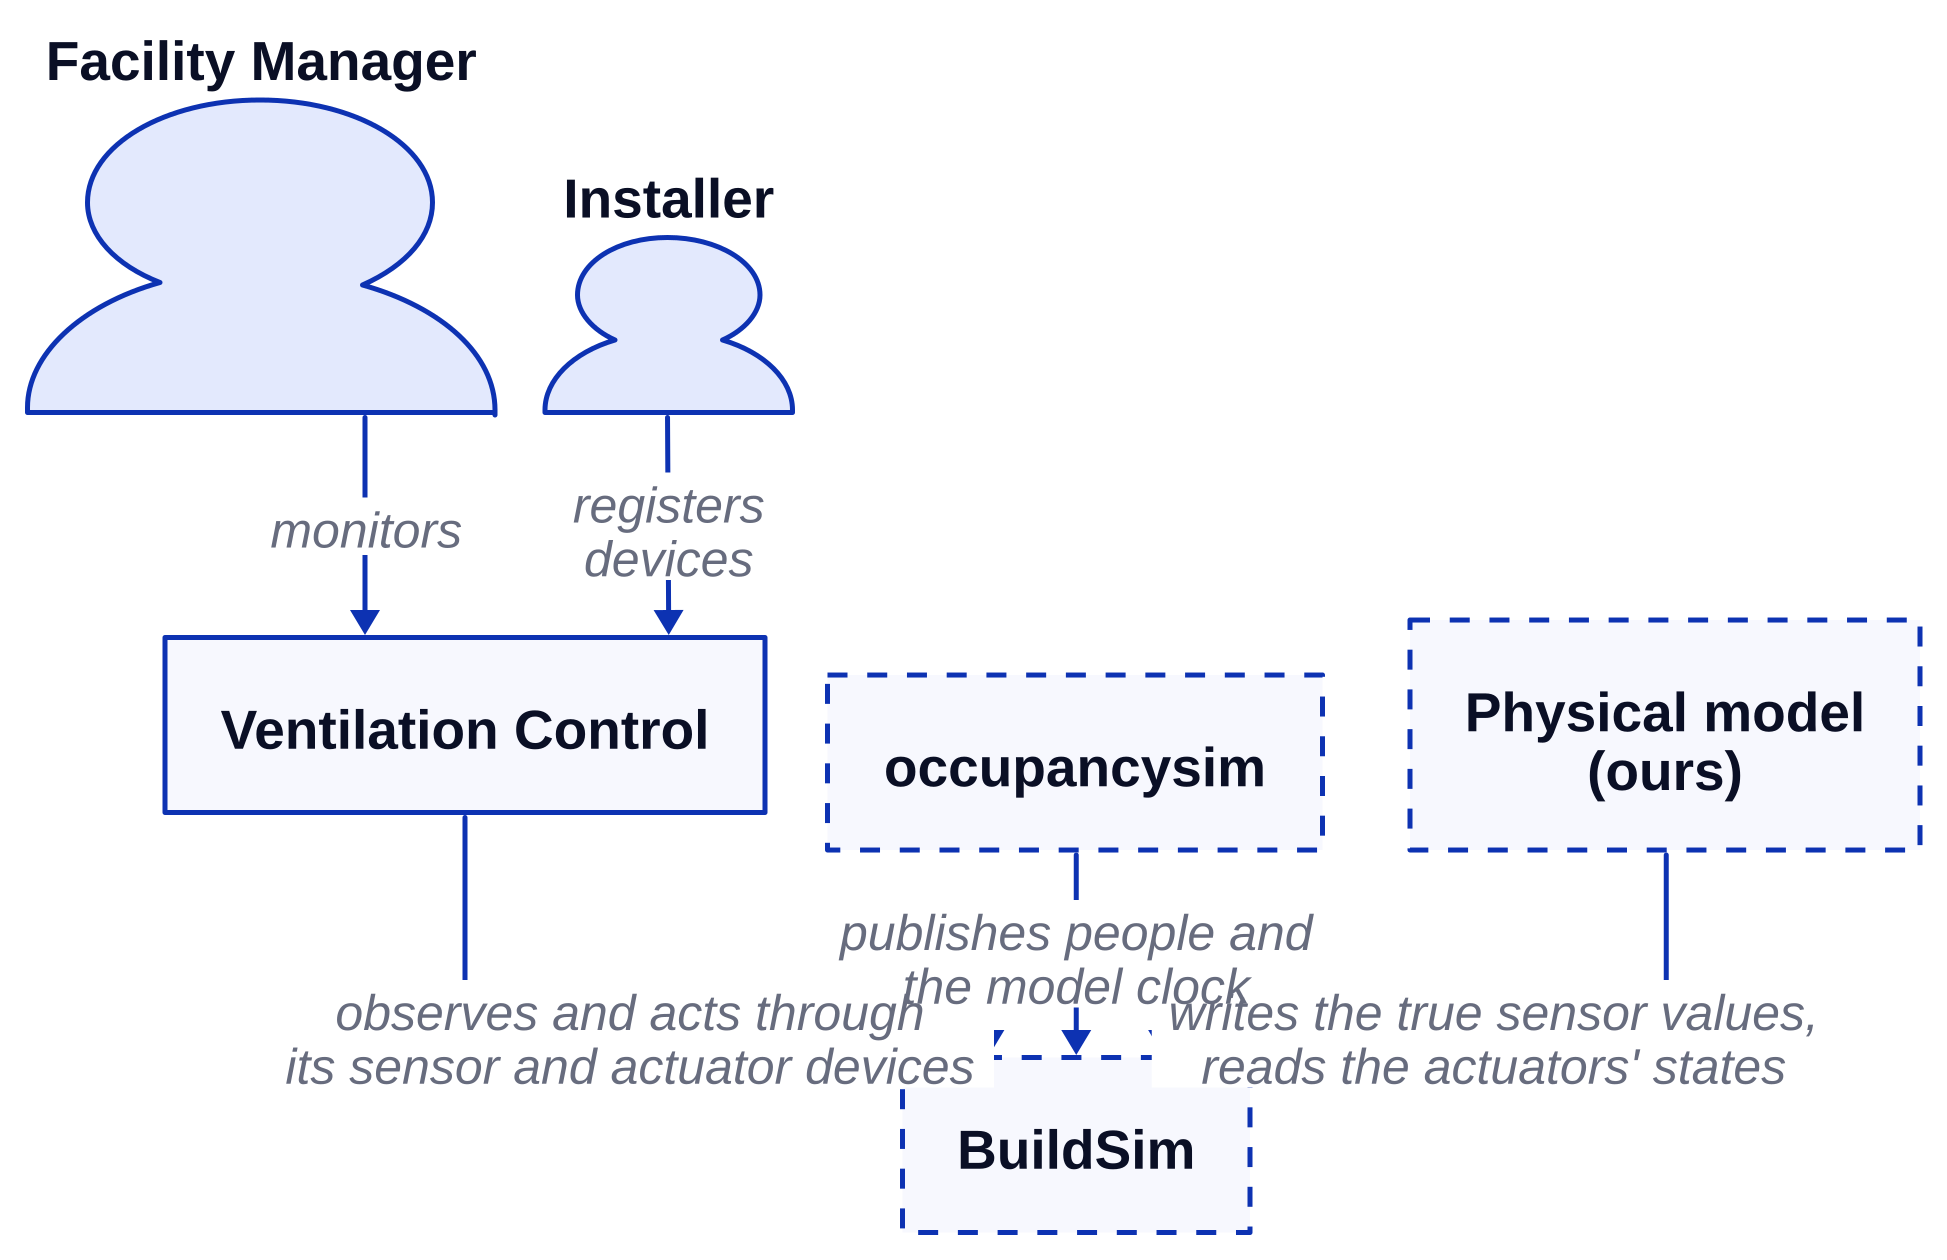
\includegraphics[width=0.76\linewidth]{figures/context.png}\end{center}

The simulated building is three things: BuildSim (course), the occupancy simulator
(course example, modified) and our physical model. They are outside the control system
on purpose: together they stand in for a real building. \emph{Ventilation Control}
touches the building only through its sensor and actuator devices. A facility manager
watches the dashboard; an installer registers devices.

\subsection{4.2 Container diagram (C4 Level 2)}

The container level is drawn as two views, because with every link in one picture the
labels are too small to read on a page. The first is the control loop and the data path.
The second is commissioning and the dashboard; boxes with the same name are the same
containers. A two-way arrow names both directions.

\widefigurewithnote{figures/container.png}{\textbf{View 1:} the control loop and the data path.}

\widefigurewithnote{figures/container-support.png}{\textbf{View 2:} commissioning and the dashboard.}

Every sensor and actuator is its own container (251 devices), so one dead device affects
one room. The occupancy simulator and the physical model talk to BuildSim and to nothing
else. A sensor device reads the true value at its place in BuildSim, adds its own
measurement error and publishes the reading on MQTT. The controller subscribes, decides,
and commands each room's actuators over REST; an actuator applies the command within its
safety limits and writes the state it has reached to BuildSim, where the physical model
reads it back. That closes the loop. Storage records every message; the dashboard (viz)
draws from the same messages. The registry holds what the installer entered: device id,
kind, room and the room's design capacity. The truth recorder (truthlog) is outside the
control system: it copies the physical model's state to a broker topic only storage may
read, for the evaluation.

\subsection{4.3 Component diagram (C4 Level 3): the controller}

\begin{center}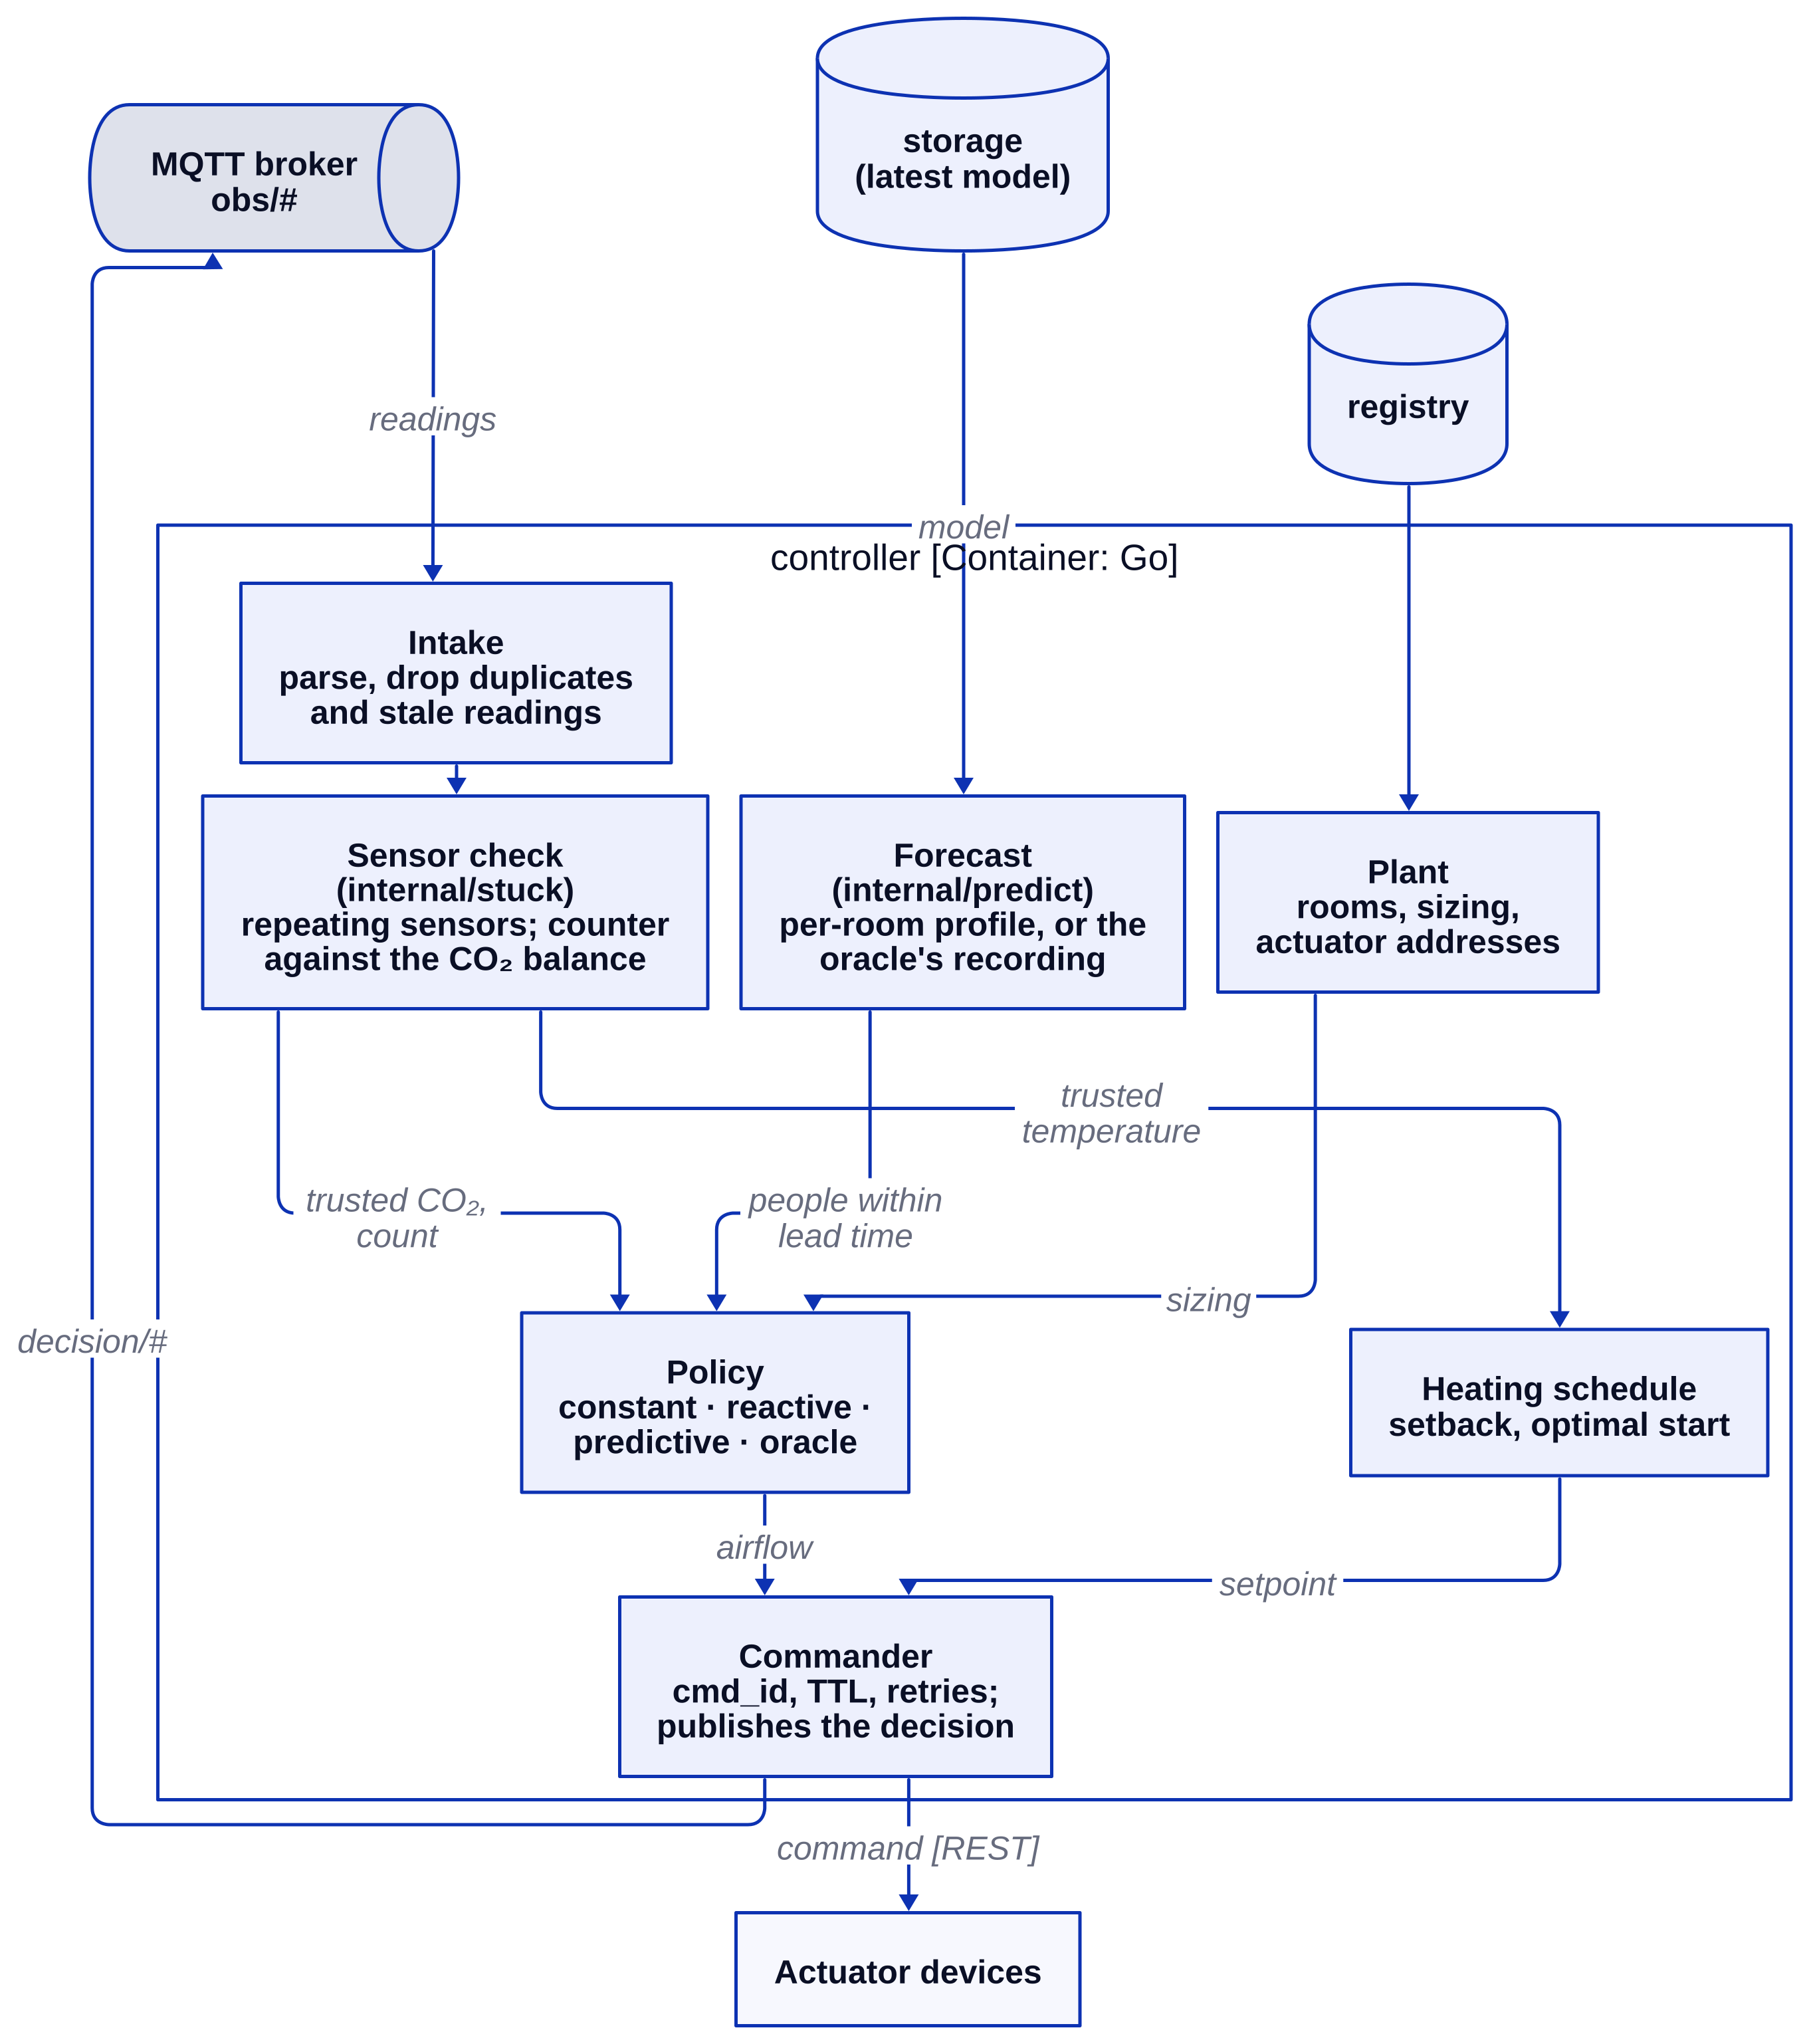
\includegraphics[width=\linewidth]{figures/component.png}\end{center}

Validation, forecast and policy sit in one process because they are one critical path
with no reason to be restarted separately. Readings pass a sensor check before the policy
sees them. The forecast is a model fetched from storage and kept in memory, so storage
may be down. The commander gives each command an id and a time to live and retries with
the same id, which the actuator treats as one command.

\subsection{4.4 Design decisions and alternatives}

\begin{longtable}[]{@{}>{\raggedright\arraybackslash}p{0.24\linewidth}>{\raggedright\arraybackslash}p{0.27\linewidth}>{\raggedright\arraybackslash}p{0.41\linewidth}@{}}
\toprule
\textbf{Decision} & \textbf{Alternatives considered} & \textbf{Why this one} \\
\midrule
\endhead
D-12 BuildSim in the middle: the two simulators talk only to BuildSim; the controller reaches it only through devices & A truth API on the physical model beside BuildSim, and the controller polling BuildSim as a fallback (built first) & It is the lab's architecture, and one representation of the building instead of two. The controller is kept from the truth by having no BuildSim address. Cost: the truth is visible in the viewer, and there is no control without the broker \\
D-1 Model time; physics steps whole model minutes from a per-minute occupancy record & Each service on its own wall-clock times factor; sampling BuildSim's occupancy & Reproducible: two runs of a day are identical. Sampling gave 99.6\,\% equal samples and made the oracle baseline unsound \\
D-2 One container per sensor; noise and faults in the device & One gateway per kind; noise in the physical model & A fault is a property of one device and can be injected on one. Cost: about 150 containers, generated \\
D-3 MQTT for readings, REST for commands & Everyone polling BuildSim & Four consumers of each reading (controller, damper, storage, dashboard). A command needs an answer, so it is a request \\
D-4 A storage service owning JSONL per run & Files shared between processes; a database server & No shared files; replayable. A history query reads the whole run, too slow for live graphs, so viz keeps its own recent copy \\
D-5 Predictor inside the controller; training as a batch job & Predictor as a service & No network hop on the control path; training off it \\
D-6 Safety in the actuator: range, rate, TTL, flow floors, \cotwo{} override & A check inside the controller & Survives a wrong or dead controller (T-10) \\
D-7 Four policies; the oracle replays a recorded run's true occupancy & Oracle reading the simulator's plans & Shows how much a perfect forecast could gain. Needs identical days (D-1) \\
D-8 Dashboard: layers and alerts in the BuildSim viewer, and a page of graphs served by viz & Grafana over storage; the viewer alone & The viewer shows now; ventilation questions are about time. One HTML file, no dependencies \\
D-10 A registry (SQLite) that devices check in with & Device lists in configuration; registering directly in BuildSim & How a building is commissioned; survives BuildSim restarting blank (T-17) \\
D-11 Stuck sensors: a run of identical readings for \cotwo{} and temperature; the counter against two bounds from the \cotwo{} balance & ``Counter unchanged while \cotwo{} moves''; estimating head-count from \cotwo{} and airflow & The first blames every healthy counter (\cotwo{} lags the count); the second needs the true airflow. The bounds hold for any airflow \\
Room set: 50 rooms & Whole building (838 rooms) & 260 containers is what one laptop runs, after two kernel settings \\
\bottomrule
\end{longtable}

\section{5. Interfaces and data contracts}

Rooms are keyed \texttt{<level>/<room>}; times are model time, RFC 3339. Full contracts with
failure behaviour are in \texttt{docs/interfaces.md} (IF-1 to IF-12).

\begin{longtable}[]{@{}>{\raggedright\arraybackslash}p{0.27\linewidth}>{\raggedright\arraybackslash}p{0.13\linewidth}>{\raggedright\arraybackslash}p{0.52\linewidth}@{}}
\toprule
\textbf{Interface} & \textbf{Owner} & \textbf{Content} \\
\midrule
\endhead
BuildSim sensor \texttt{sim-clock-minutes} & occupancy simulator & Clock, and people per room for the last ten model minutes \\
BuildSim \texttt{PUT /api/sensors/\{id\}/value} & physics & True value at every sensor, once per minute; the minute itself, last, at the clock device \\
MQTT \texttt{obs/<level>/<room>/<kind>} & each sensor & The reading, QoS 1; consumers drop exact repeats of \texttt{(sensor\_id, seq)} \\
MQTT \texttt{time/model} & clock device & The building's minute, on change and every real second \\
REST \texttt{POST /rooms/\{l\}/\{r\}/command} & actuator & \texttt{202} target, \texttt{200} duplicate, \texttt{409} expired, \texttt{422} invalid \\
BuildSim \texttt{PUT /api/actuators/\{id\}/state}; MQTT \texttt{state/...} & each actuator & The state it has reached \\
MQTT \texttt{decision/...}, \texttt{event/...} & controller; actuators & Every decision with its mode and reason; overrides and expiries \\
MQTT \texttt{truth/...} & truthlog & True room state per minute; the broker lets only storage read it \\
REST storage, registry & & History and models; devices, rooms, check-in \\
\bottomrule
\end{longtable}

{\scriptsize\begin{verbatim}
obs/level0/A1519/co2  {"run_id":"eval-predictive-v4","sensor_id":"co2-0041","room":"level0/A1519","kind":"co2",
                       "value":439,"unit":"ppm","model_time":"2026-09-21T08:21:00Z","seq":1789978860}
command               {"cmd_id":"a99e...","value":308.0,"unit":"l/s","issued_at":"2026-09-21T10:15:00Z",
                       "ttl_s":300,"reason":"predictive: CO2 612 ppm, 25 people within 12 min"}
\end{verbatim}}

\section{6. Simulating the sensor values (the physical model)}

Per room, with $n$ people, airflow $q$, volume $V$, floor area $A$:
\[ V\frac{dC}{dt} = n\,G + q\,(C_\text{out}-C), \qquad
   c_A A\,\frac{dT}{dt} = U\!A\,(T_\text{out}-T) + \rho c_p\,q\,(T_\text{sup}-T) + 100\,\text{W}\cdot n + P_\text{rad} \]
with $G$ = 0.005\,l/s of \cotwo{} per person, $C_\text{out}$ = 420\,ppm, ceiling 2.7\,m,
$T_\text{out}$ = 8\,\textdegree C, supply air 18\,\textdegree C, and a radiator of
60\,W/m\textsuperscript{2} that is fully on 0.5\,K below its setpoint. Both equations are
solved exactly over each model minute. The loop closes because $q$ and the setpoint are
\emph{the states the actuators report in BuildSim}, not the commands. The energy proxy is
fan power (1.5\,kW per m\textsuperscript{3}/s), heating the supply air, and radiator power.

Ventilation is sized by the Swedish workplace rule: $q_\text{design}$ = 7\,l/s per person
of design capacity + 0.35\,l/s\,m\textsuperscript{2}; the maximum is 1.5 times that. A full
room at design flow settles near 1000\,ppm, which is why the maximum is higher.

Occupancy comes from the course's simulator: a seeded plan per day with staff in offices,
lectures in four slots in rooms drawn at random, breaks at 09:45 and 14:30, and night
guards. We changed it in three logged ways: fixed 5-second steps, a record of people per
room at every whole minute, and publishing that record and its clock into BuildSim.
A sensor reading is the true value plus Gaussian noise (a $\pm$1 miscount in 10\,\% of
readings for the counter), and injected faults: stuck, dropout, drift.

\section{7. Autonomous services and data pipeline}

\subsection{7.1 The autonomous service}

\textbf{Policies.} \emph{Constant}: design flow on weekdays 07--18, the minimum otherwise.
\emph{Reactive}: flow rises linearly from the minimum at 600\,ppm to the maximum at
1000\,ppm. \emph{Predictive}: the larger of the reactive flow and the workplace-rule flow
for the people expected, where ``expected'' is the larger of the count now and the
forecast within the room's lead time (its time constant, 10 to 30 minutes).
\emph{Oracle}: the same with the true future occupancy of a recorded run. Heating is the
same under all four: 21\,\textdegree C on weekdays 07--18, 18\,\textdegree C otherwise,
starting early enough to be warm at 07:00.

\textbf{The learned part} is a per-room profile: for each weekday quarter-hour, the
80th percentile across training days of that slot's occupancy. Within a day a slot's
value is the 75th percentile of its readings, not the maximum: taking the maximum let the
counter's occasional false ``1'' make the model expect someone in 86\,\% of all slots,
nights included, and cost 25\,\% more energy until we found it. Without a model the
policy runs as reactive and says so.

\textbf{Stuck sensors} keep reporting, so silence does not reveal them. A \cotwo{} or
temperature sensor is noisy, so 5 (or 12) identical readings in a row cannot be chance:
those are the shortest runs a healthy 50-room building produces less than once in 100
days. A counter legitimately reads 0 for hours, so it is checked against the \cotwo{}
balance instead: with $x$ the \cotwo{} above outdoor, $x$ cannot rise faster than
$nG/V$, nor stay below $(nG/q_\text{max})(1-e^{-t\,q_\text{max}/V})$, whatever the
airflow. A counter that has not moved and breaks either bound is distrusted.

\subsection{7.2 The data pipeline}

Sensors publish on MQTT. Storage appends every reading, truth record, decision, event and
actuator state to one JSONL file per stream and run, and serves history, exports and
models over HTTP; nothing is deleted. The trainer is a batch job that reads a training
run from storage and stores a model, which the controller picks up. The controller keeps
only the latest readings; the dashboard keeps a week of minutes in memory and refills
from storage after a restart.

\section{8. Behaviour}

\subsection{8.1 Key scenario: a lecture room fills}

\widefigure[1.0]{figures/dynamic.png}

The order of steps 3 to 6 is the point: the physical model writes the minute to the
clock device \emph{after} that minute's values, and sensors sample when the clock shows a
new minute, so each reading belongs to its minute. At factor 120 every one of 150 sensors
delivered 120 of 120 readings (T-42).

\subsection{8.2 Process lifecycle: a damper}

\begin{center}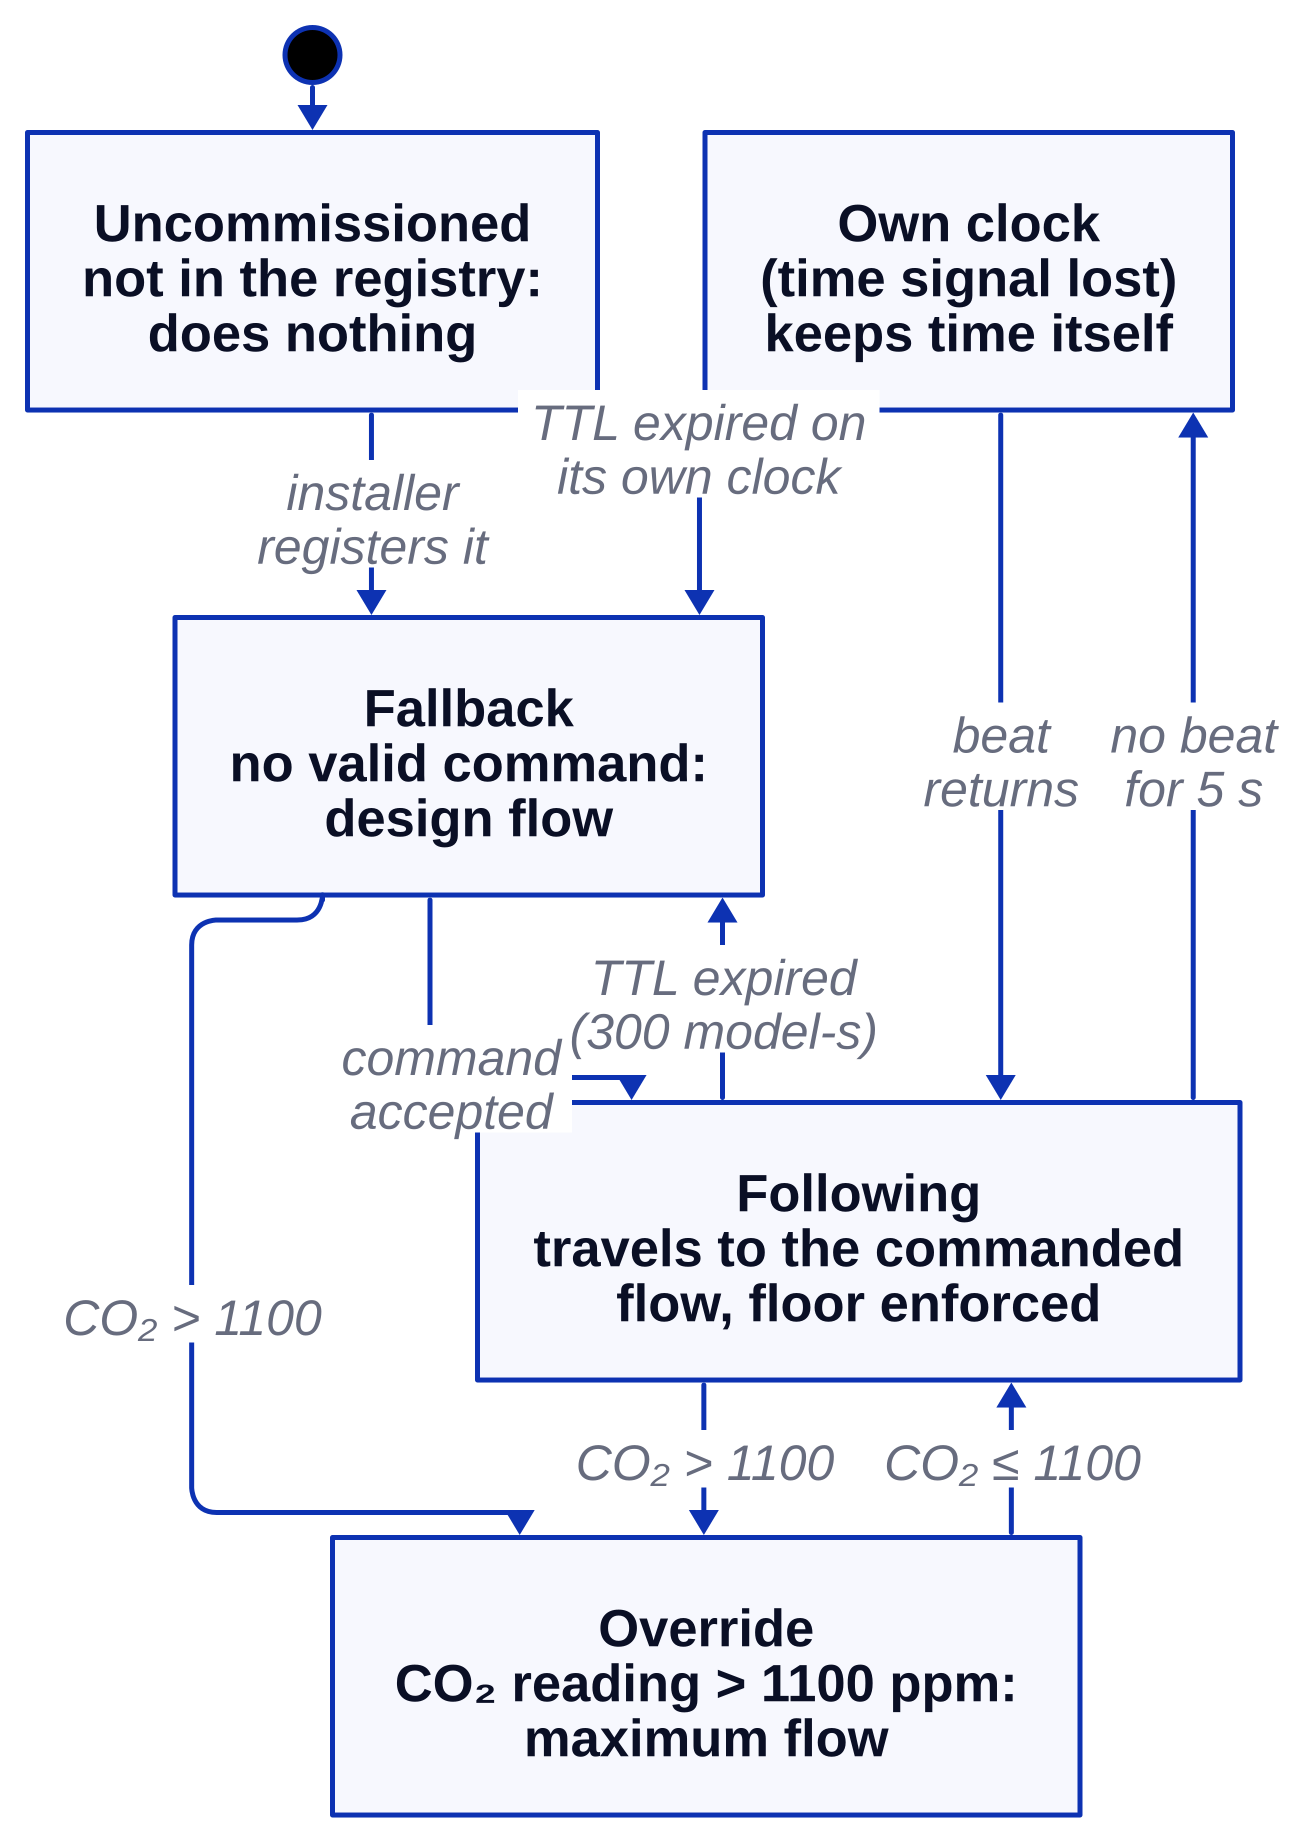
\includegraphics[width=0.52\linewidth]{figures/state.png}\end{center}

A damper without a valid command is at design flow. Commands expire after 300 model
seconds, so a silent controller, sensor or broker returns the room to design flow
without anyone deciding it. If the time signal itself stops, the damper keeps time at the
last known speed so that the expiry still happens.

\section{9. Deployment and component view}

\widefigure{figures/deployment.png}

Everything runs as containers on one laptop under one compose network, generated from
the installation list. In a building, each device container would be a device, and the
grouping in the figure is where the rest would run: sensing, validation of commands and
the safety limits at the edge, where they must survive the network; prediction, storage
and the dashboard on a building server; training offline.

\section{10. Test plan}

43 tests; the full table with every result is \texttt{docs/test-plan.md}. Unit tests
(\texttt{go test}, 20 packages) cover the model, noise, policies, actuator, detector and
each piece of the data path. The live tests are three scripts, each its own run id.

\begin{longtable}[]{@{}>{\raggedright\arraybackslash}p{0.09\linewidth}>{\raggedright\arraybackslash}p{0.30\linewidth}>{\raggedright\arraybackslash}p{0.10\linewidth}>{\raggedright\arraybackslash}p{0.41\linewidth}@{}}
\toprule
\textbf{ID} & \textbf{Test} & \textbf{Req.} & \textbf{Result} \\
\midrule
\endhead
T-09/10 & Sensor drifts above 1100\,ppm with the controller killed & FR-6 & Damper at its maximum, 315.6\,l/s, with no controller running \\
T-12 & Counter frozen at 53 during a lecture & FR-7 & Not blamed while the room was full; found 14 minutes after it emptied; flow 408 to 37\,l/s \\
T-13 & \cotwo{} sensor stopped & FR-7 & Command expired after 5 minutes; damper to design flow; cleared on return \\
T-36 & \cotwo{} sensor frozen; temperature sensor frozen & FR-7 & Found after 5 and 12 readings. 12 people in the room; true \cotwo{} peaked at 571\,ppm \\
T-17 & BuildSim restarted blank & FR-11 & 253 pieces of equipment back in 7.8\,s; readings in 9.1\,s \\
T-23 & Each of nine services killed in turn & NFR-6 & Loop closed in all rooms within 2\,s of restart. \textbf{No container restarted by itself} (Podman) \\
T-24, T-40 & Broker stopped; clock device stopped & NFR-6 & All 100 actuators expired their commands on their own clocks; design flow; recovered alone \\
T-21 & Command to damper movement & NFR-4 & 93\,\% within one model minute; \textbf{95th percentile 2: missed} \\
T-22 (stress) & Simulation speed doubled until readings are lost & NFR-5 & 100\,\% at factor 120, 79\,\% at 240, 25\,\% at 960 \\
T-25 & Same week under four policies and two data paths & NFR-7 & 360\,500 truth records, every head-count equal \\
T-27 & Controller's login reads the truth topic & scope & Receives nothing; has no BuildSim address \\
T-38 & Stuck-sensor detector over fault-free runs & FR-7 & No false alarm in 1.44 million readings of each kind \\
T-43 & What storage holds of a run & FR-8 & Every reading from the first minute; found a bug that discarded a run's readings \\
\bottomrule
\end{longtable}

\section{11. Evaluation and results}

A training week (14--18 Sep 2026) under the reactive policy, then the held-out week
21--25 Sep once per policy, at 120 times real time. The four runs saw the same people in
every room at every minute, so differences are the policies'.

\begin{longtable}[]{@{}lrrrr@{}}
\toprule
 & \textbf{Constant} & \textbf{Reactive} & \textbf{Predictive} & \textbf{Oracle} \\
\midrule
\cotwo{} $\leq$ 1000\,ppm, occupied (NFR-1) & 94.5\,\% & 100.0\,\% & 100.0\,\% & 100.0\,\% \\
\quad in lecture rooms & 65.2\,\% & 100.0\,\% & 100.0\,\% & 100.0\,\% \\
Occupied minutes above 1000\,ppm & 745 & 4 & 0 & 0 \\
Peak \cotwo, ppm & 1167 & 1028 & 963 & 963 \\
20--24\,\textdegree C, occupied (NFR-2) & 100.0\,\% & 100.0\,\% & 100.0\,\% & 100.0\,\% \\
Energy, kWh per week & 15\,231 & 6\,284 & 6\,519 & 6\,372 \\
Saving against constant (NFR-3) & & 59\,\% & 57\,\% & 58\,\% \\
\bottomrule
\end{longtable}

\begin{center}
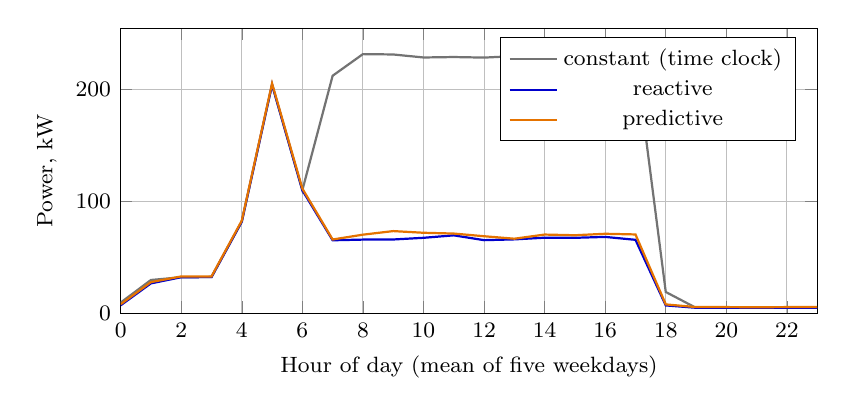
\begin{tikzpicture}
\begin{axis}[width=0.86\linewidth,height=5.2cm,xlabel={Hour of day (mean of five weekdays)},ylabel={Power, kW},
  xmin=0,xmax=23,ymin=0,grid=major,legend pos=north east,legend style={font=\footnotesize},
  tick label style={font=\footnotesize},label style={font=\footnotesize}]
\addplot[black!55,thick] coordinates {(0,9.4) (1,29.6) (2,32.1) (3,32.2) (4,81.7) (5,204.1) (6,109.8) (7,212.1) (8,231.4) (9,231.1) (10,228.4) (11,228.8) (12,228.3) (13,229.6) (14,229.5) (15,227.6) (16,228.7) (17,229.3) (18,18.9) (19,4.7) (20,4.7) (21,4.7) (22,4.7) (23,4.7)};
\addplot[blue!80!black,thick] coordinates {(0,7.0) (1,26.6) (2,32.1) (3,32.2) (4,81.7) (5,204.1) (6,109.8) (7,65.1) (8,65.7) (9,65.8) (10,67.3) (11,69.5) (12,65.2) (13,65.9) (14,67.4) (15,67.3) (16,68.1) (17,65.5) (18,6.9) (19,4.8) (20,4.7) (21,4.7) (22,4.7) (23,4.7)};
\addplot[orange!90!black,thick] coordinates {(0,7.9) (1,27.7) (2,32.8) (3,32.8) (4,82.6) (5,205.2) (6,111.3) (7,65.8) (8,70.1) (9,73.3) (10,71.8) (11,71.1) (12,68.7) (13,66.5) (14,70.2) (15,69.6) (16,70.9) (17,70.3) (18,7.8) (19,5.4) (20,5.4) (21,5.3) (22,5.4) (23,5.4)};
\legend{constant (time clock),reactive,predictive}
\end{axis}
\end{tikzpicture}
\end{center}

\textbf{Reading.} A time clock costs two and a half times as much and still fails: a
full lecture room settles around 1000\,ppm at design flow, and anyone in an office
outside 07--18 sits at the night minimum. Reactive control already does almost
everything: four minutes over the limit in a week, at the lowest energy. A perfect
forecast (oracle) removes those four minutes for 1.4\,\% more energy; our predictor gets
the same air for 3.7\,\% more. That small gap between reactive and oracle is itself the
result: the dampers reach full flow in minutes and lecture rooms catch up fast, so
there is little for anticipation to win. The peak at 05:00 in the figure is the same
under every policy: radiators bringing the rooms back from the night setback.

\textbf{Where the numbers are weak.} The forecast foresaw 87\,\% of arrivals in common
rooms, with false alarms in 23\,\% of quiet moments, and \emph{none} in lecture rooms:
the simulator puts each lecture in a random room, so a room has no pattern to learn. It
is one seed and one week. The building is a model we wrote, so the result says as much
about its time constants as about the controllers. NFR-4 is missed at the 95th
percentile (T-21), and above factor 120 readings are lost (T-22).

\textbf{A check on the rework.} The same week had been measured on the first data path.
After rebuilding it, reactive, predictive and oracle came out at 6\,284, 6\,519 and
6\,372\,kWh against 6\,282, 6\,521 and 6\,370: the architecture changed, the behaviour did
not.

\section{12. Dashboard}

The dashboard is one process, viz, with two faces. In the BuildSim 3D viewer it
publishes five room layers (\cotwo, people counted, people expected, airflow as a share
of the room's maximum, temperature) and the current alerts. On its own page
(port 8060) it shows the building and each room over time, up to a week back.

\begin{center}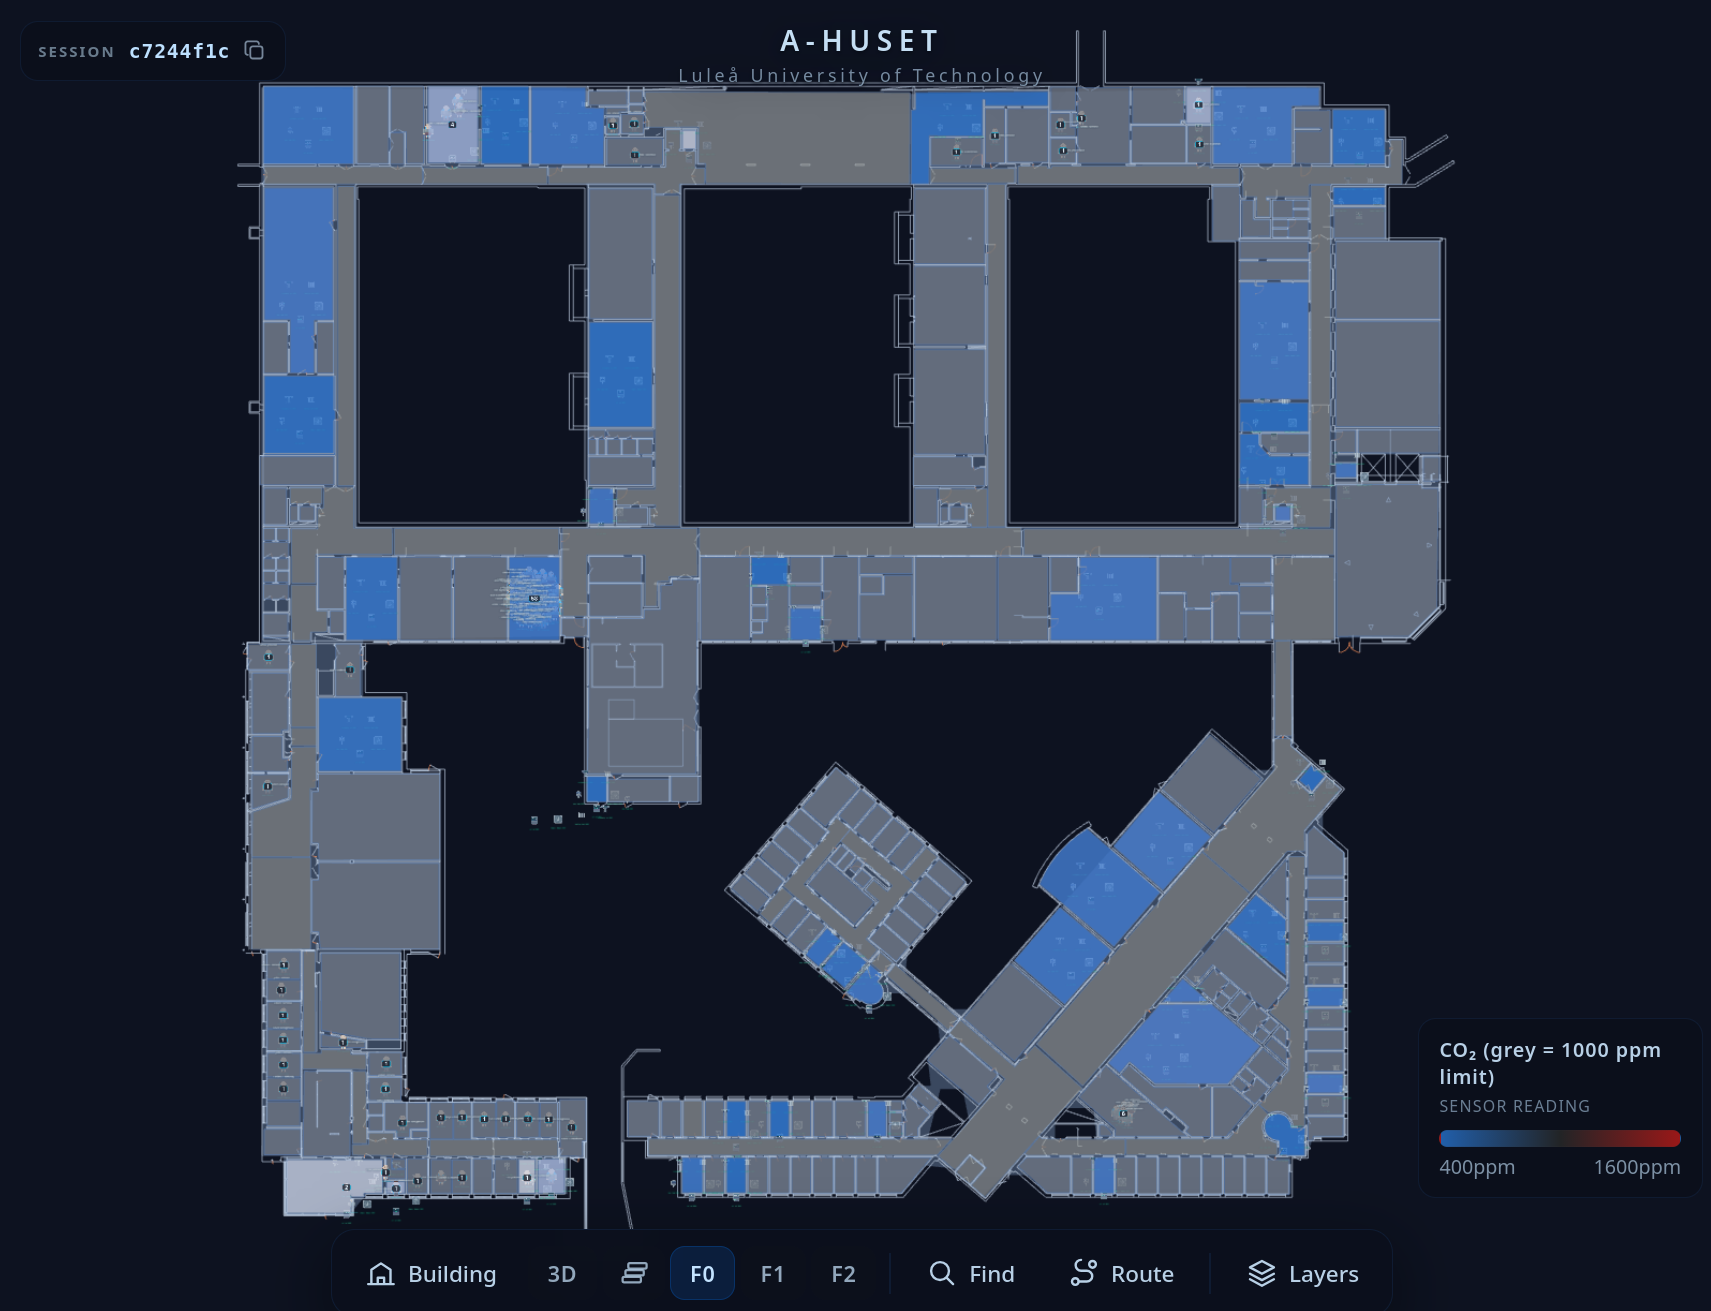
\includegraphics[width=\linewidth]{figures/3d-view.png}\end{center}

The first figure is the viewer on level 0 with the \cotwo{} layer: each room we
instrument is coloured by its sensor's latest reading, on a scale from 400 to
1600\,ppm with grey at the 1000\,ppm limit, so blue is air well under the limit.

\begin{center}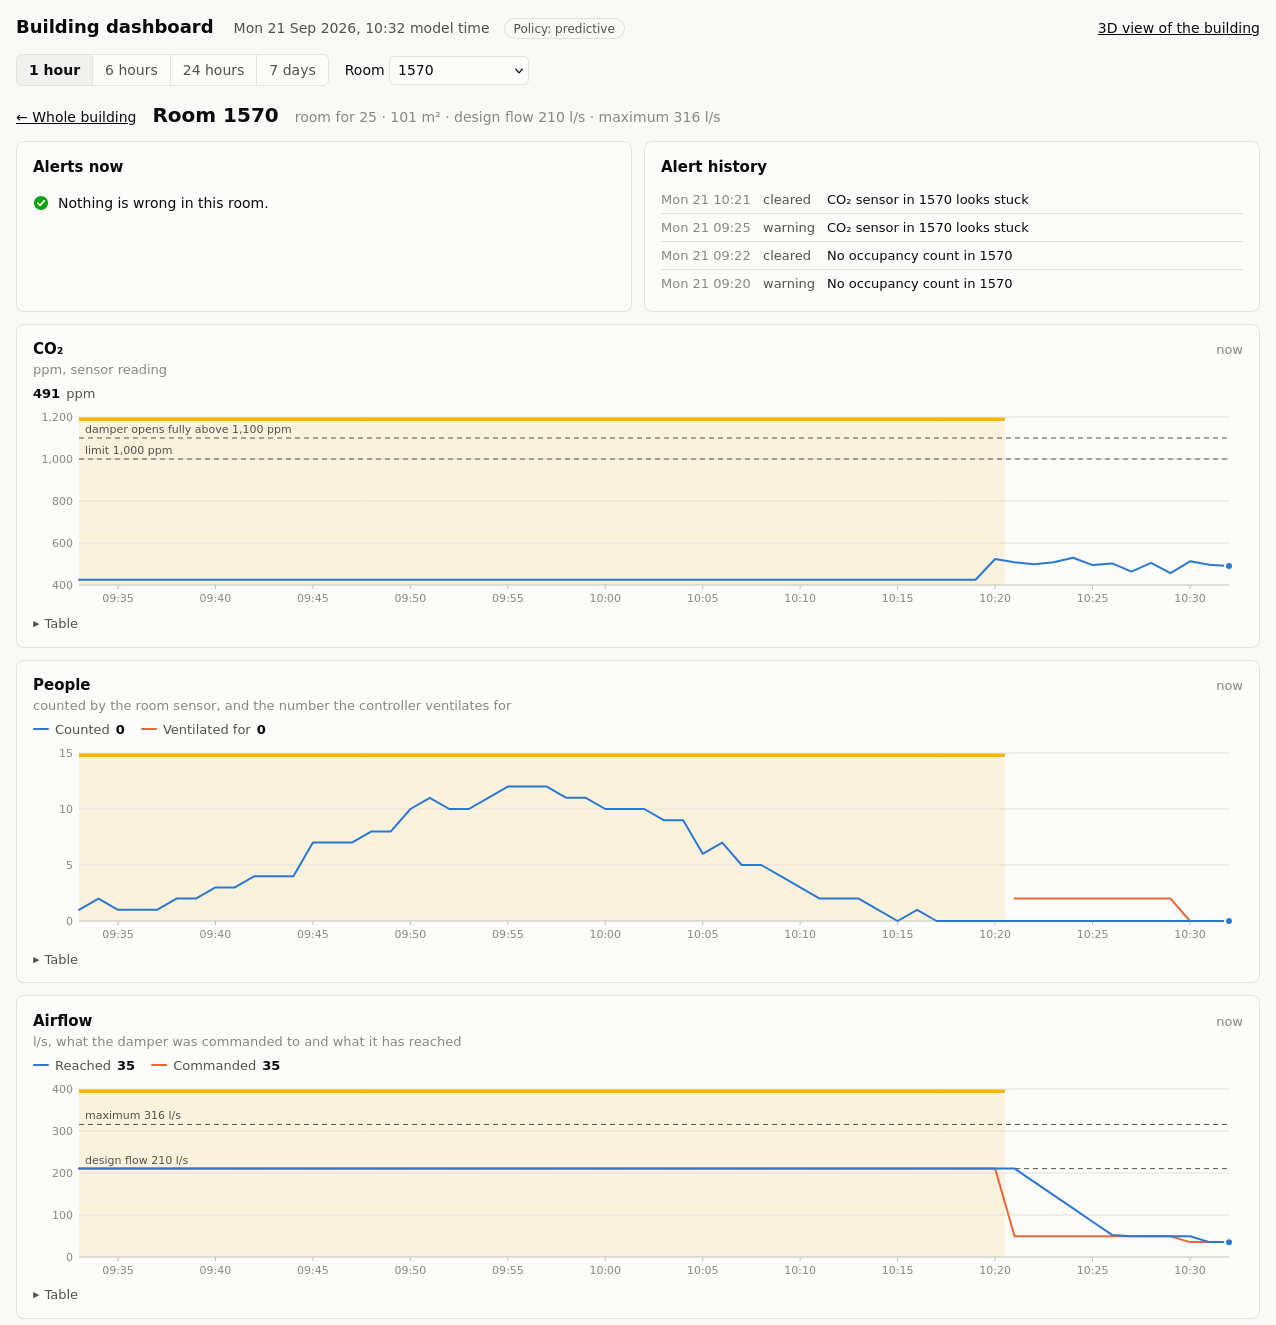
\includegraphics[width=\linewidth]{figures/dashboard-room.png}\end{center}

The second figure is a room whose \cotwo{} sensor was frozen at 09:20: the flat reading, the alert
period shaded, the damper held at design flow while up to 12 people came and went, and
its rate-limited return when the sensor was repaired. Everything shown arrived on MQTT
from a sensor, the controller or an actuator: the dashboard shows the building as the
control system knows it, never the truth.

\section{13. Risks and critical reflection}

\textbf{We built the wrong data path first.} For ten days the physical model had its own
API and the controller could read BuildSim. We noticed two days before the deadline and
rebuilt it. It cost a night of reruns and bought the lab's architecture, exact sampling,
and one finding we would otherwise have missed: storage had been discarding readings
whenever time moved backwards, which the new start-up order exposed.

\textbf{The prediction earns little here.} It spends 3.7\,\% more energy to remove four
minutes above the limit. With slower dampers or tighter limits it would matter more; a
lecture timetable as an input would let it foresee lectures, which it cannot now.

\textbf{The truth is visible in BuildSim.} Clicking a device in the viewer shows the true
value. The controller is kept from it by configuration and by the broker's access list,
not by authentication, which BuildSim does not have.

\textbf{Known limits.} No control without the broker (the actuators then take safe,
wasteful defaults). A counter stuck on a small number is not found: below about a
quarter of a room's capacity its \cotwo{} is inside the sensor noise. A drifting sensor
is not detected. A killed container is not restarted automatically under Podman. Devices
do not authenticate to the registry. The heating's warm-up rate is assumed, not learned.

\textbf{On working with an AI assistant.} Most code was written with one. The review log
(\texttt{docs/review-log.md}) records each piece of its advice that was wrong and how we
caught it: the data path above, a baseline that ventilated all night, a training rule
that turned sensor noise into people. Each was caught by measuring, not by reading the
code.

\textbf{With more time:} a second seed and a longer evaluation; the lecture timetable;
learning the warm-up rate; a per-run blank BuildSim; network isolation of BuildSim from
the controller.

\end{document}
